%        File: hw1.tex
%     Created: Sat Apr 06 10:00 AM 2013 P
% Last Change: Sat Apr 06 10:00 AM 2013 P
%
\documentclass[11pt]{article}

\usepackage{amsmath, amssymb, amsthm, cite, graphicx, float, mathrsfs, commath, dsfont, bbm, bm, setspace,lipsum}
\usepackage[mathscr]{eucal}
\usepackage[sc]{mathpazo}
\linespread{1.05}
%\usepackage{setspace}
%\onehalfspacing
\usepackage[margin=1in, top=.8in, left=.8in]{geometry}
\usepackage{color}

% new commands
\DeclareMathOperator*{\argmin}{arg\,min}
\DeclareMathOperator{\sgn}{sgn}
\newcommand{\E}{\mathrm{E}}
\newcommand{\Var}{\mathrm{Var}}
\newcommand{\Cov}{\mathrm{Cov}}
\newcommand{\Cor}{\mathrm{Cor}}
\newcommand{\id}{\operatorname{id}}
\newcommand{\diag}{\operatorname{diag}}
\newcommand{\Id}{\operatorname{Id}}
\newcommand{\tr}{\operatorname{tr}}
\newcommand{\Q}{\mathbb{Q}}
\newcommand{\C}{\mathbb{C}}
\newcommand{\R}{\mathbb{R}}
\newcommand{\Z}{\mathbb{Z}}
\newcommand{\F}{\mathbb{F}}
\newcommand{\N}{\mathbb{N}}

\newcommand{\indep}{\rotatebox[origin=c]{90}{$\models$}}

% 524 commands
%\newcommand{\norm}[1]{\| #1 \|}
\DeclareMathOperator{\spn}{span}
%\newcommand{\spn}{\operatorname{span}}
\newcommand{\onenorm}[1]{\| #1 \|_{L^1(\mathbb R^d)}}
\newcommand{\twonorm}[1]{\| #1 \|_{L^2(\mathbb R^d)}}

% 534 commands
\renewcommand{\Re}{\text{Re\,}}
\renewcommand{\Im}{\text{Im\,}}

\begin{document}
\pagestyle{empty}
\hfill Abraham Engle

\hfill Stat 571

\hfill \today
\begin{enumerate}
 	%1
	\item Let $\sigma=\mathrm{expit}$. The first method uses the mean and variance from the model
	\begin{align*}
		Y_i &\sim_{indep} \mathrm{Bin}(T_i,p_i) \\
		p_i &= \sigma(\beta_1 + \beta_3\mathrm{trtbas}(i))
	\end{align*}
	for $i=1,2,\dotsc,59$. The second uses the mean and variance from the model
	\begin{align*}
		Y_{ij} &\sim_{indep} \mathrm{Bern}(p_{ij}) \\
		p_{ij} &= \sigma(\beta_1 + \beta_3\mathrm{trtbas}(i))
	\end{align*} 
	for $j=1,2,\dotsc,T_i$ and $i=1,2,\dotsc,59$. The point estimates are the same because the score equations are the same (which just follows from the fact that the log-likelihood of the binomial $Y_i$ is a constant multiple away from the sum of the individual Bernoulli likelihoods). However, the second model we are modeling plain vanilla logistic regression on the counts $Y_{ij}$, not accounting for the clustering present. This forces independence across \emph{all} observations. On the other hand, the first model assumes independence across only the binomial observations. \\ \\We know from last quarter that sandwich estimation under these two models provides consistent estimation of the variance provided observations are uncorrelated (pg 57 of the textbook). In the second model, we do not have uncorrelated counts within any cluster $\{Y_{i1},\dotsc,Y_{iT_i}\}$, so we do not, in general, have consistent estimates from this sandwich. On the other hand, we do have have this assumption from the progabide setup in (a), so I would choose these standard error estimates to report in favor of the model-based approach, which were much closer to the estimating equations produced from the Bernoulli model.
	%2
	\item I used INLA for both parts (a) and (b) and JAGS and INLA for part (c).
	\begin{enumerate}
		\item Using INLA in R, the following posterior means and 95\% credible intervals for the random effects $b_i$ are given from the complete case data set:
		\begin{figure}[H]
		\centering
			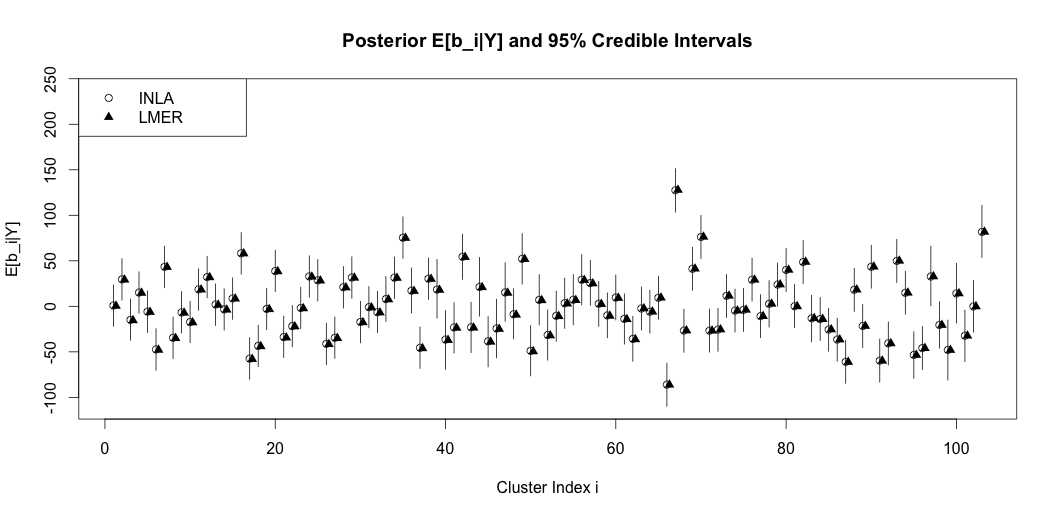
\includegraphics[scale=0.4]{Rplotp21}	
		\end{figure}
		The posterior mean and 95\% credible intervals for the fixed effects are
% latex table generated in R 3.2.3 by xtable 1.8-0 package
% Tue Mar 15 13:17:00 2016
\begin{table}[H]
\centering
\begin{tabular}{rrrr}
  \hline
 & 0.5quant & 0.025quant & 0.975quant \\ 
  \hline
(Intercept) & 224.53 & 212.97 & 236.05 \\ 
  trt & 5.87 & -12.30 & 24.02 \\ 
  time & 7.17 & 4.87 & 9.48 \\ 
  trt:time & -1.46 & -4.96 & 2.03 \\ 
  sigY & 24.82 & 26.91 & 23.11 \\ 
  sigb & 37.14 & 44.48 & 32.36 \\ 
   \hline
\end{tabular}
\end{table}
\item First I plot diagnostics for normality
	\begin{figure}[H]
		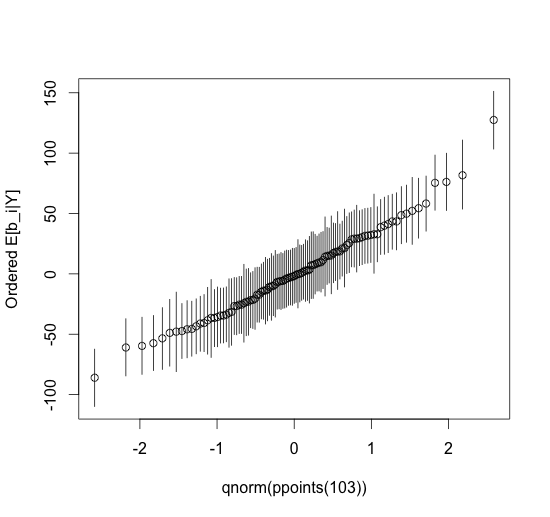
\includegraphics[scale=0.4]{Rplotp2b1}
		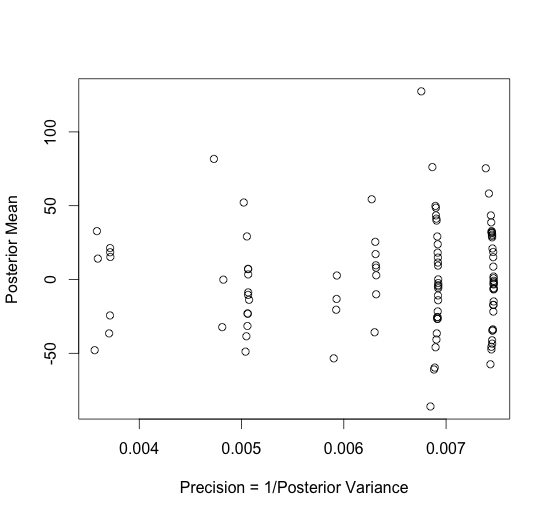
\includegraphics[scale=0.4]{Rplotp2b2}
	\end{figure}
	There is a strong linear association between the ordered posterior means and normal quantiles, except for what might be a small amount of a characteristic heavy-tailed S shape described on slide 3.82. Since there are so few extreme posterior means relative to most of the activity in the center, I do not think we should be seriously concerned.
	\\  The second plot displays the posterior mean against the precision. We have a wide range of means for larger precision (=smaller variance), but I think it might be the case that there are just relatively few posterior samples at the lower precisions, so I am again not seriously concerned. \\ \\ 
	Next I move on to mean model diagnostics, comparing the results with plain-vanilla LMM mean model diagnostics:
	\begin{figure}[H]
		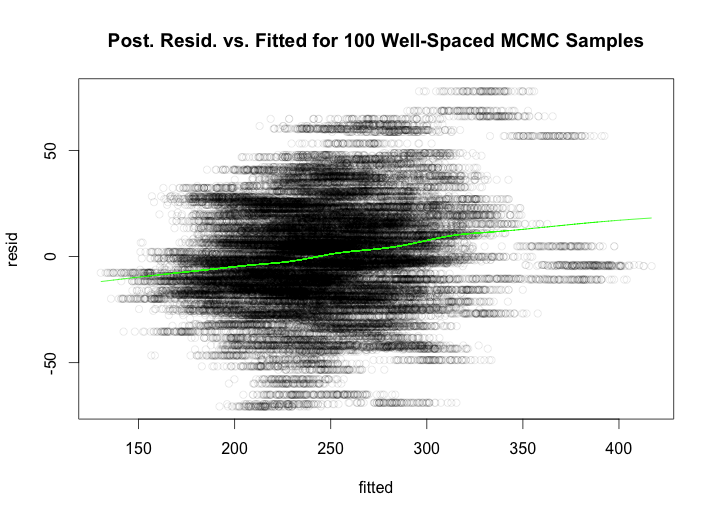
\includegraphics[scale=0.4]{Rplotp2b3}
		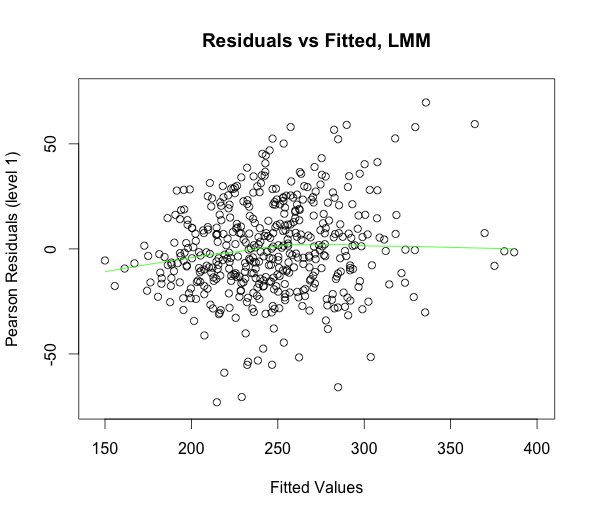
\includegraphics[scale=0.4]{Rplotp2b4.png}
	\end{figure}
	It looks to me like when sampling from the posterior distribution, we obtained  a few higher fitted values with corresponding higher residuals, which did not appear in the LMER case. I next assess individual cluster influence with leave one out diagnostics. I plot the cluster index against estimates of the fixed effects with 95\% intervals.
	\begin{figure}[H]
		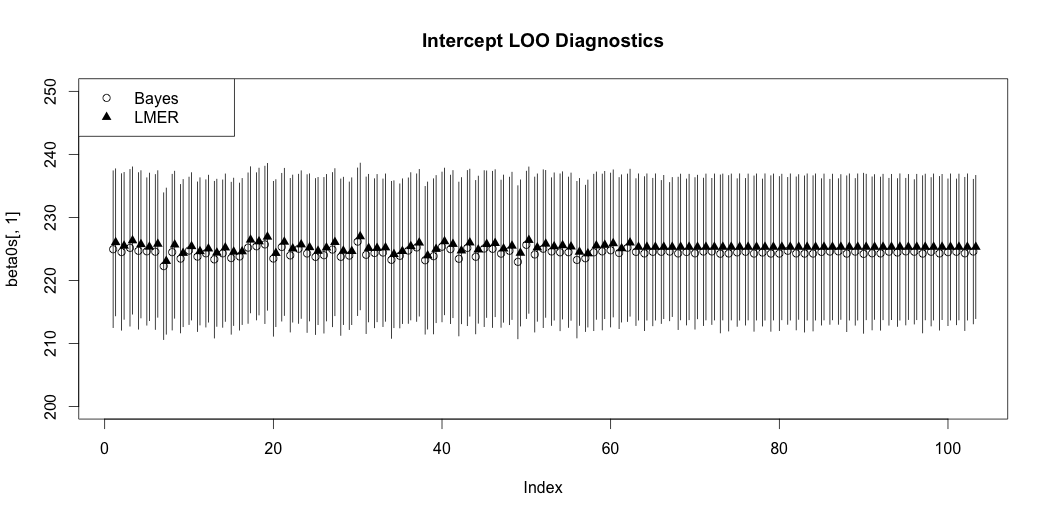
\includegraphics[scale=0.4]{Rplotp2b5}
		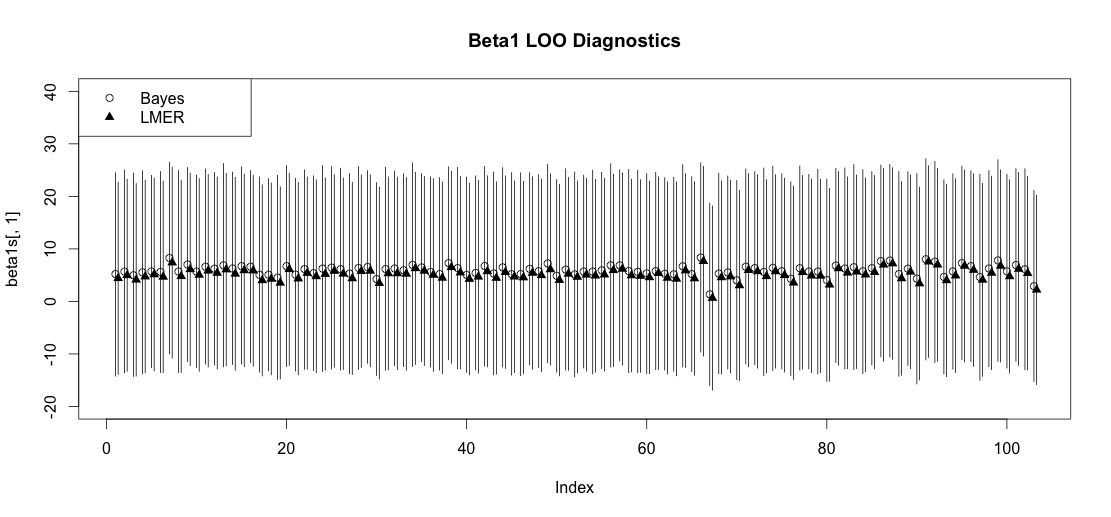
\includegraphics[scale=0.4]{Rplotp2b6}
	\end{figure}
	\begin{figure}[H]
		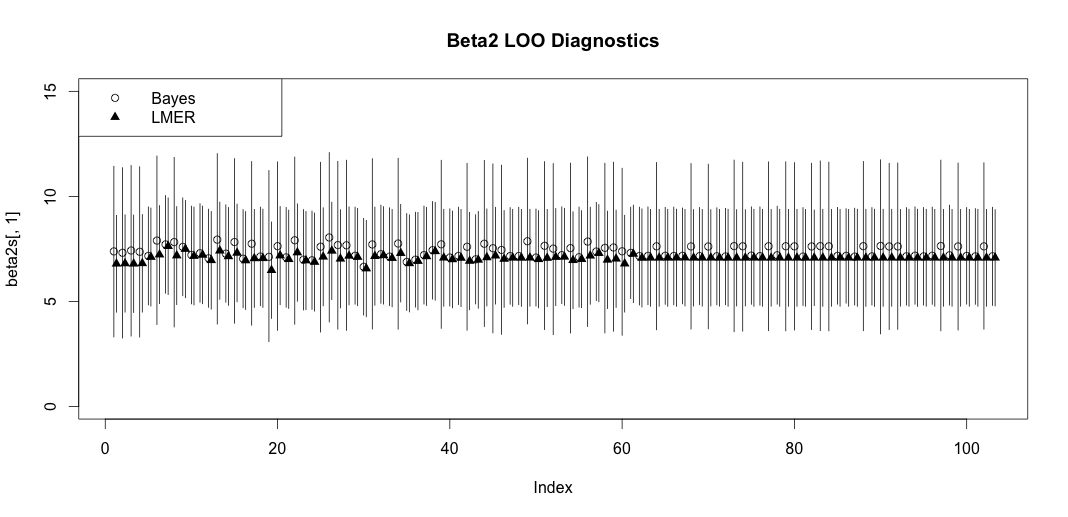
\includegraphics[scale=0.4]{Rplotp2b7}
		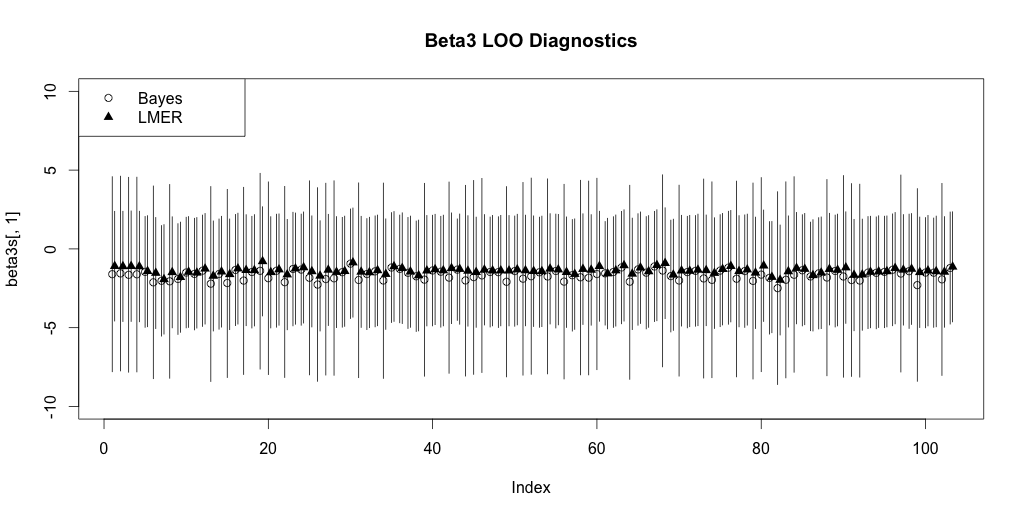
\includegraphics[scale=0.4]{Rplotp2b8}	
	\end{figure}
 In the last two figures, the confidence bands for INLA vary quite widely depending on which cluster is left out, but LMER does not display this behavior. I think this behavior combined with the mean model behavior on the previous page causes some concern. 
\item Using MCMC in part (a) on the complete cases, we can obtain a few well-spaced samples from the posterior distribution for the random effects $\widetilde{b}_i$ and the fixed effects $\widehat{\beta}$. With these samples, we can impute missing values from the fitted model $X_{ij}^T\widehat{\beta}+Z_{ij}^T\widetilde{b}_i$. If we did this $K$ times, we are in the setup on slide 2.148 to analyze each ``complete" data set and use Rubin's rules on all $K$ analyses.
\end{enumerate}
\newpage
	%3
	\item {\setstretch{2.0}
	 The authors are interested in models which specify either conditional or marginal means of outcomes $Y_{ij}$ on random effects $U_i$ and fixed effects $X_i$, taken to be independent of one another. Modeling conditional means of outcomes takes the form given in equation (1) as
	\[
		g(E[Y_{ij}|U_i]) = K[z_i^TU_i, \mu(X_i,\beta)],
	\]
	where conditioning on the covariate $X_i$ is implicit throughout the paper. In class we mainly studied this structure for $K[z_i^TU_i, \mu(X_i,\beta)] = z_i^TU_i + \mu(X_i,\beta),\; \mu(X_i,\beta) = X_i^T\beta$ with $g=id$ giving LMM and with $g$ an arbitrary link we obtained GLMM. From the conditional mean $E[Y|U,X]$ we obtain the marginal mean via the tower law $E[Y|X]=E[E[Y|U,X]]$. The authors emphasize that when studying longitudinal data, marginal and conditional parameters derived from the previous models do not always share the same interpretation. The paper provides some general designs where parameters are identical or have identical interpretations.
	
	Section 2 begins similar to how we began chapter 3, where the model in (5) is equivalent to the model in slide 3.8. As we saw on slide 3.9 and as the authors state, this is an example where the marginal mean is simply $\mu$, compared to the conditional mean $\mu+U$. The authors then note that this holds in general for additive $K$ and $g=id$, provided the random effects have mean zero and are independent of the covariates. Three more examples of the so-called additive random effect case are summarized in 2.1.1, where marginal distributions that arise from conditionally specified distributions $Y_{ij}|U_i$ are presented. 2.1.2 describes in detail the third example, a model with conditionally Poisson-distributed data with an identity link. 
	
	 2.2 deals with additive $K$, a log-link, and independence of covariates and random effects. We discussed this case in slide 3.113 when $\mu(X_i,\beta)=X_i^T\beta$. In general, the authors write that as long as we have finite first moment $E[|Y|]<\infty$, the marginal mean is the conditional plus a constant. This is exactly the content of the third equation in slide 3.113, where we obtained a closed form for the expectation with the moment generating function of the normal distribution. The authors emphasize that an analogous result holds for any distribution on the random effects, not just normality and linear $\mu$. They go on to give three examples within this framework, one of which is slide 3.113. They continue the detailed example of the previous section instead using a log link.
	
	 2.3 gives a more subtle example of the relationship between conditional and marginal means using the probit link. For logit links and additive normal random effects, the authors argue that marginal mean does not have a closed form, and numerical procedures confirm that coefficients $\beta$ from the marginal mean become ``attenuated" by a factor given on page 3.16 of the paper. For random effects with certain exponential densities, however, there are conditional links for which the integrals can be evaluated and from which we obtain marginal links. These marginal links proved to be computationally intractable, and the theory behind these random effects distributions was an open area of research at the time. 
	 
	 Finally, the authors conclude with a discussion about dependence between the random effects and covariates. In this case, the marginal density is $f(y|X) = \int_U f(y|u,X)\dif F(u|X)$, where before the measure reduced to $\dif F(u)$. The authors mention an alternative marginalized random effects model and that if we incorrectly assume $\Var(b_i) = G$ which does not depend on $X_i$, we introduce bias in parameter estimates. In the case of correlated covariates and random effects, the methodology from a problem known as the omitted covariate problem applies, where we treat the random effect as an omitted covariate in the corresponding marginal model.
	\par}
	%4
\newpage
	\item
		\begin{enumerate}
			%a
			\item Following slide 3.206 using a single sample with $n=10^4$, the estimates and standard errors are
			\begin{table}[H]
			\centering
			\begin{tabular}{cr|c|c}
				\hfill & Truth & LMM REML & GEE (Exchangeable) \\
				\hline
				$\widehat{\beta}_0$ & 1 & 0.99696 & -0.0396 \\
				$\widehat{\beta}_1$ & -1 & -0.99851 & -1.09200 \\
				$\widehat{\beta}_2$ & 0.5 & 0.50805 & -0.2181 \\
				$\frac{\widehat{\sigma}_b^2}{\widehat{\sigma}^2_b + \widehat{\sigma}_Y^2}$ & 0.8 & 0.7981277 & 1.115 (!!!) \\				
			\end{tabular}
			\end{table}
			To save some time for computation, I reduced the sample size to $n=10^3$ and increased the number of replications of the data generating mechanism to $K=10^3$. Histograms of coefficient estimates are
			\begin{figure}[H]
				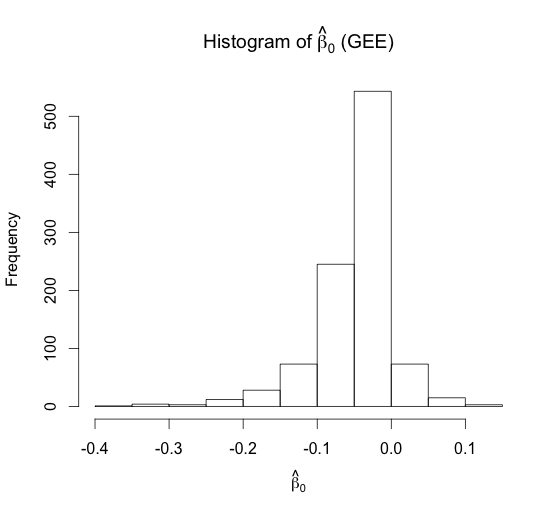
\includegraphics[scale=0.4]{Rplot4b0GEE}
				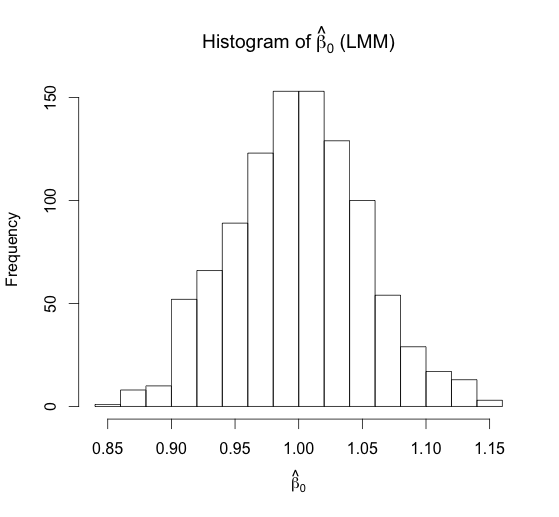
\includegraphics[scale=0.4]{Rplot4b0LMM}
				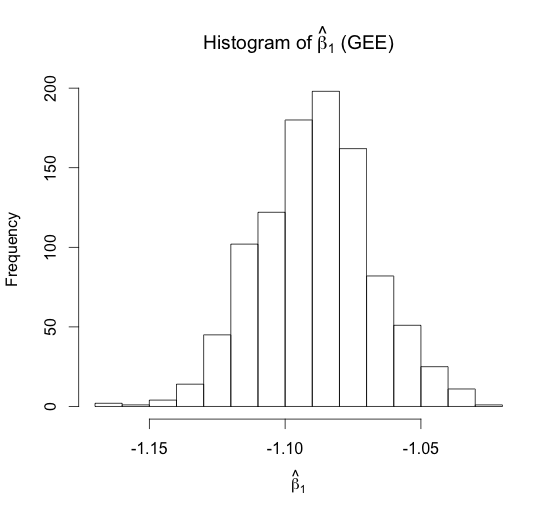
\includegraphics[scale=0.4]{Rplot4b1GEE}
				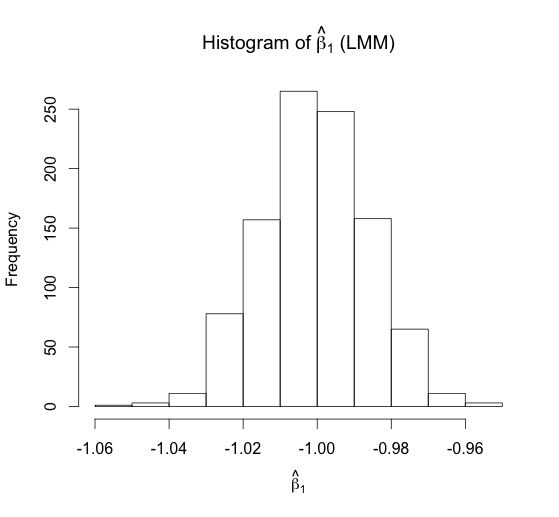
\includegraphics[scale=0.4]{Rplot4b1LMM}
				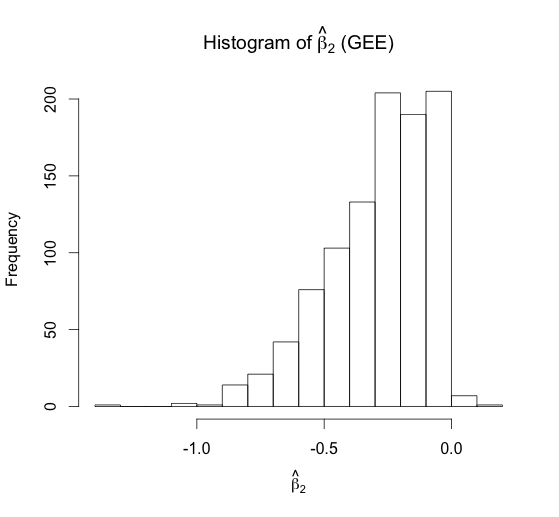
\includegraphics[scale=0.4]{Rplot4b2GEE}
				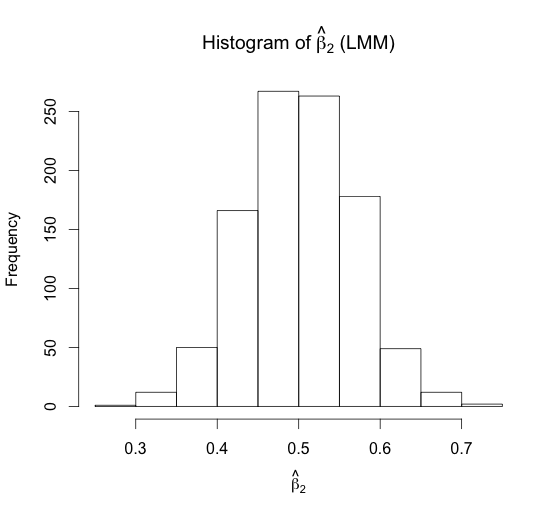
\includegraphics[scale=0.4]{Rplot4b2LMM}
			\end{figure}
			Empirical coverage probabilities for all three coefficients in the GEE case are 0\%, and in the LMM are $95.5\%, 94.6\%, $ and $95.1\%$ for $\widehat{\beta}_0, \widehat{\beta}_1, \widehat{\beta}_2$ respectively.
			%b
			\item As we've seen on slide 2.135, if we have missing data the GEE applied to the observed responses solves the estimating equation
			\[
				\frac{1}{n}\sum_{i=1}^n D_i^T V_i^{-1}\diag(1-M_{ij})(Y_i-\mu_i) = 0_p,
			\]
			and solutions to this estimating equation in general are biased for the parameters of interest. Whenever data is MCAR, we obtain consistent estimates from these equations.\\ \\
			On the other hand, using the likelihood-based approach in LMM together with the fact that we have data MAR, slide 3.203 argues that the joint density $f(Y^{(o)},M|X) \propto f(Y^{(o)}|X)$, hence we can maximize the left-hand side using complete case analysis and a likelihood approach with LMM. Since the two are just constant multiples off, we obtain valid inference on the parameters.
		\end{enumerate}
	%5
	\item In each problem, I generate data from the mechanism 1,000 times and compute Wald-type p-values described in slide 3.25. I compute what proportion of $p$-values are $<0.05=\alpha$, which gives an empirical proportion of times we would reject the null hypothesis falsely in favor of $\beta_1\neq 0$.
	\begin{enumerate}
		\item The nominal proportion is about 7.9\%. A histogram of the p-values is
		\begin{figure}[H]
		\centering
			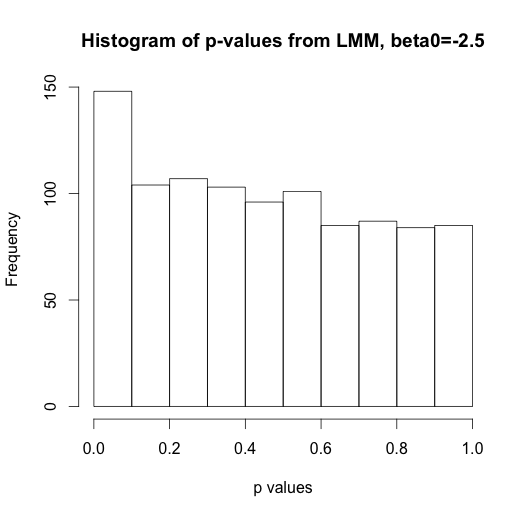
\includegraphics[scale=0.4]{Rplotp5a}
		\end{figure}
		
		\item Fitting a GLMM with a logistic link, the empirical proportion is about 6.9\%. A histogram of the p-values is
		\begin{figure}[H]
		\centering
			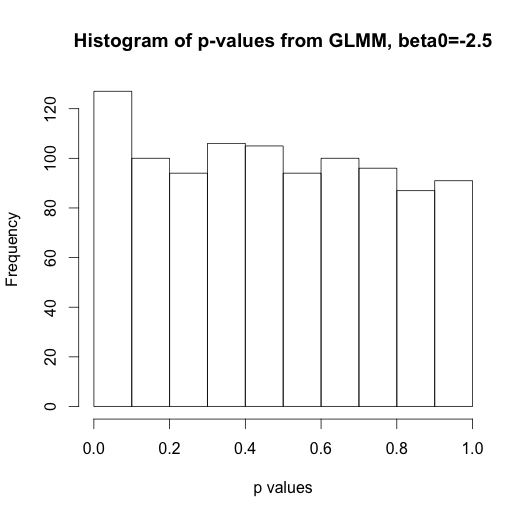
\includegraphics[scale=0.4]{Rplotp5b}
		\end{figure}
		
		\item With $\beta_0=-0.75$, the empirical proportion of rejections of the null is about $0.053\%$ and $0.054\%$. Histograms of the p-values are
		\begin{figure}[H]
			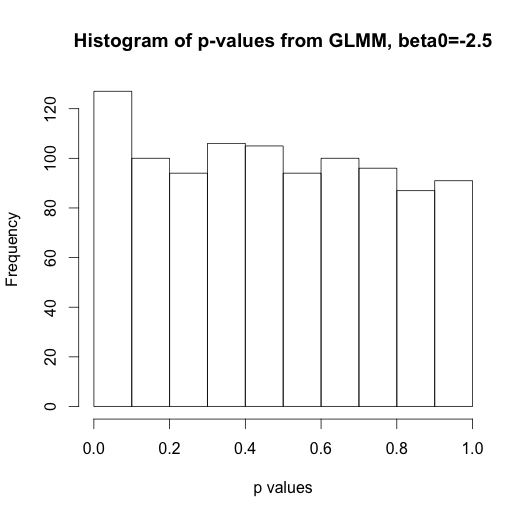
\includegraphics[scale=0.4]{Rplotp5b}
			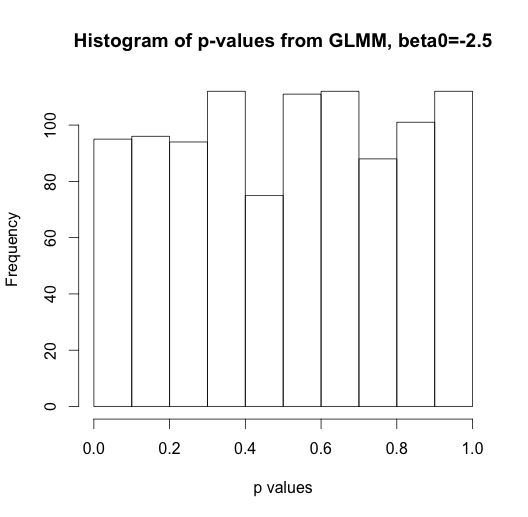
\includegraphics[scale=0.4]{Rplotp5c}
		\end{figure}
		
		\item For the GLMM in both cases, we assume i.i.d. normal random effects with mean zero and independent Bernoulli outcomes conditional on the random effects. We try to fit linked mean model $E[Y_{ij}|b_i,X_{ij},Z_i]=\sigma(\beta_0+b_i+\beta_1X_{ij}+\beta_2Z_i)$. The data generating mechanism almost completely agrees with this setup. We generated outcomes $Y_{ij}$, conditional on a normal random effect with mean zero and confounder $Z_i$, as independent Bernoulli trials. The only difference is that the outcomes are independent of the covariates $X_{ij}$. I believe GLMM accurately fits the model and the empirical proportions are quite close to what we expect, possibly some Monte Carlo error prevents us from obtaining exactly $0.05\%$ rejection.
		
		Similarly, LMM assumes i.i.d. random normal effects with mean zero and attempts to fit, conditional on the random effect $b_i$, a mean $E[Y_{ij}|b_i,X_{ij},Z_i]=\beta_0+b_i+\beta_1X_{ij}+\beta_2Z_i$. Obviously we have misspecified the mean since the outcomes $Y_{ij}$ were known to be binary. What's more, the LMM assumes intra-cluster variability $\Var(Y_{ij}|X_{ij},b_i)=\sigma^2_Y$, which is completely determined from the mean in the Bernoulli case. Furthermore, the intra-cluster correlation we already know to be zero. 
		\\ \\
		Roughly, for an average cluster (so $b_i=0$ and $Z_i = p$) the data generating mechanism draws independent Bernoulli random variables with success probabilities $\sigma(\beta_0+\beta_2p)\approx 0.1066906$ and 0.4073334 for $\beta_0=-2.5$ and $\beta_0=-0.75$ respectively. The average cluster also draws $X_{ij}\sim \mathrm{Bin}(2,\sigma(\theta_0+\theta_1p) \approx 0.1645165)$. On average, we mostly see $X_{ij}=0$ since $P(X_{ij}=0|Z_i=p) \approx 0.7$. I am not really sure why LMM performs so well, but I want to say that it is mostly seeing $X_{ij}=0$ and i.i.d. draws from a Bernoulli with success explained mostly by $Z_i$. Therefore fitting a non-zero coefficient $\widehat{\beta}_1$ does not affect inference strongly enough, so we fail to reject $\beta_1=0$ quite often for the LMM. I believe this is even more pronounced when the probabilities of success for the outcomes is closer to 50\%, which helps explain why LMM performs even closer to GLMM.
		\end{enumerate}
	%6
	\item Typos
		\begin{enumerate}
			\item Slide 3.61, $\epsilon_i || X_i=x_i, Z_i= z_i$ should have the second vertical bar removed.
			\item Slide 2.135 line 4. The last expectation is missing a ``$]$"
			\item Slide 2.135 line 4. The first expectation has an extra $|X_{ij}$. Should just read $P[M_{ij}=0|X_{ij},Y_{ij}]$.
			\item Slide 2.135 line 9 should read $P[M_{ij}|X_{ij}]$ since we assumed MCAR.
			\item Slide 1.27 line -4, the first sum is missing the upper decoration $n$
			\item Slide 1.28 indented equation I believe $\bm{x}_i$ should be $\bm{x}_i^T$ since the previous line viewed $\bm{x}_i$ as a column vector when writing $\bm{x}_i^T\beta$.
			\item Slide 1.52 the second indented equation has an extra comma inside
			\item Slide 3.25 the first indented equation has the transpose on the wrong side, the right version is on 3.24 since $X_i\in \R^{n_i\times p}$.
			\item Slide 3.26 same comment as above.
			\item Slide 3.43 The denominator of the REML likelihood in the quadratic form should have a $V^{-1}$, the determinant to the left should also be modified.
			\item Slide 3.113 the second indented equation has an extra expectation on the right. I think we are just saying
			\[
				\log(E[Y_{ij}|X_{ij},Z_{ij},b_i]) = Z_{ij}^Tb_i + X_{ij}^T.
			\]
			The equation immediately below it has another expectation in the middle quantity as well.
		\end{enumerate}
\end{enumerate}
\newpage
R Code
\begin{verbatim}
	library(geeM)
library(R2WinBUGS)
library(lme4)
library(nlme)
library(mcmc)
library(rjags)
library("INLA")
library("sandwich")
setwd("~/Dropbox/UW2015-2016/Win2016/571/hw10")
setwd("C:\\Users\\aengl_000\\Dropbox\\UW2015-2016\\Win2016\\571\\hw10")
###########
#problem 1#
###########
seiz.l = read.table("seizl.txt", header=TRUE, sep=" ")
Ti <- aggregate( subset(seiz.l, t>1)$y, by=list(seiz.l$id), sum )[,2]
Yi1 <- subset(seiz.l, t==8)$y
trtbas <- subset(seiz.l, t==8)$trt # treatment at time j=1

glm1 <- glm(cbind(Yi1, Ti-Yi1) ~ trtbas , family=binomial)
round( cbind( est=coef(glm1), rob.se=sqrt(diag(vcovHC(glm1, "HC0"))) ) , 2)

Ylong <- rep( rep(c(1,0),each=59), c(Yi1, Ti-Yi1) )
trtbaslong <- rep( c(trtbas,trtbas), c(Yi1, Ti-Yi1) )
glm2 <- glm(Ylong ~ trtbaslong, family=binomial)
round( cbind( est=coef(glm2), rob.se=sqrt(diag(vcovHC(glm2, "HC0"))) ) , 2)

###########
#problem 2#
###########
prob2DF <- read.table("hw10q2.csv", header=TRUE, sep=",")
prob2DF$index = 1:nrow(prob2DF)
lmer1 <- lmer(y~trt+time+trt*time + (1 |id) ,data=prob2DF)
hyperprior <- list(theta=list(prior="loggamma",param=c(0.1,0.1)))
fixedprior <- list( mean.intercept=0, prec.intercept=0.0001,
                    mean=0, prec=0.0001 )
formula1 <- y ~ trt + time + trt*time +
  f(id,model="iid",hyper=hyperprior) #+ f(index,model="iid", hyper=hyperprior)
set.seed(10)
inla1 <- inla(formula1, family="gaussian", data=na.omit(prob2DF), control.fixed=fixedprior, 
control.family = list(prior="loggamma",param=c(0.1,0.1)))

#model reporting
inlaRANEF = round(inla1$summary.random$id[,c(2,4,6)],2)
plot(1:103,inlaRANEF[,1], pch=1, ylim=c(min(inlaRANEF[,2]),max(inlaRANEF[,3])),
main="Posterior E[b_i|Y] and 95% Credible Intervals", xlab="Cluster Index i", ylab="E[b_i|Y]")
points((1:103)+0.3,ranef(lmer1)$id[,1],pch=17)
for(i in 1:103)
{
  segments(x0=i, y0=inlaRANEF[i,2], y1=inlaRANEF[i,3])
}
legend("topleft", legend=c("INLA", "LMER"), pch=c(1,17))

# fixed effects
xtable(round(rbind(inla1$summary.fixed[,c(4,3,5)],1/sqrt(inla1$summary.hyperpar[,c(4,3,5)])),2))

#diagnostics
ordered = order(inla1$summary.random$id[,2]) #just order the posterior means of the b_i
x = qnorm(ppoints(103)) #need these
y = inla1$summary.random$id[ordered,2]
lower = inla1$summary.random$id[ordered,4]
upper = inla1$summary.random$id[ordered,6]
plot(x,y,ylim=c(min(lower),max(upper)), xlab="qnorm(ppoints(103))", ylab="Ordered E[b_i|Y]")
for(i in 1:103)
{
  segments(x0=x[i], y0=lower[i], y1=upper[i])
}
plot(inla1$summary.random$id[,3]^(-2), inla1$summary.random$id[,2],
     xlab="Precision = 1/Posterior Variance", ylab="Posterior Mean") #WHAT DOES THIS SHOW

#now for LOO
set.seed(1)
beta0s = matrix(0,nrow=103,ncol=3)
beta1s = beta0s
beta2s = beta0s
beta3s = beta0s
beta0sLMER = beta0s
beta1sLMER = beta0s
beta2sLMER = beta0s
beta3sLMER = beta0s
for(i in 1:103)
{
  tempDF = subset(na.omit(prob2DF),id!=i)
  inlaLOO <- inla(formula1, family="gaussian", data=tempDF, control.fixed=fixedprior, control.family = list(prior="loggamma",param=c(0.1,0.1)))
  lmerLOO <- lmer(y~trt+time+trt*time + (1 |id) ,data=tempDF)
  beta0s[i,] = as.numeric(inlaLOO$summary.fixed[1,c(1,3,5)])
  beta1s[i,] = as.numeric(inlaLOO$summary.fixed[2,c(1,3,5)])
  beta2s[i,] = as.numeric(inlaLOO$summary.fixed[3,c(1,3,5)])
  beta3s[i,] = as.numeric(inlaLOO$summary.fixed[4,c(1,3,5)])
  beta0sLMER[i,] = summary(lmerLOO)$coefficients[1,1]
  +c(0,-1,1)*1.96*summary(lmerLOO)$coefficients[1,2]
  beta1sLMER[i,] = summary(lmerLOO)$coefficients[2,1]
  +c(0,-1,1)*1.96*summary(lmerLOO)$coefficients[2,2]
  beta2sLMER[i,] = summary(lmerLOO)$coefficients[3,1]
  +c(0,-1,1)*1.96*summary(lmerLOO)$coefficients[3,2]
  beta3sLMER[i,] = summary(lmerLOO)$coefficients[4,1]
  +c(0,-1,1)*1.96*summary(lmerLOO)$coefficients[4,2]
}
plot(beta0s[,1],ylim=c(200,250),main="Intercept LOO Diagnostics")
points((1:103)+0.3,beta0sLMER[,1],pch=17)
for(i in 1:103)
{
  segments(x0=i, y0=beta0s[i,2], y1=beta0s[i,3])
  segments(x0=i+0.3, y0=beta0sLMER[i,2], y1=beta0sLMER[i,3])
}
legend("topleft", pch=c(1,17), legend=c("Bayes", "LMER"))

#beta1:
plot(beta1s[,1],ylim=c(-20,40),main="Beta1 LOO Diagnostics")
points((1:103)+0.3,beta1sLMER[,1],pch=17)
for(i in 1:103)
{
  segments(x0=i, y0=beta1s[i,2], y1=beta1s[i,3])
  segments(x0=i+0.3, y0=beta1sLMER[i,2], y1=beta1sLMER[i,3])
}
legend("topleft", pch=c(1,17), legend=c("Bayes", "LMER"))

#beta2:
plot(beta2s[,1],ylim=c(0,15),main="Beta2 LOO Diagnostics")
points((1:103)+0.5,beta2sLMER[,1],pch=17)
for(i in 1:103)
{
  segments(x0=i, y0=beta2s[i,2], y1=beta2s[i,3])
  segments(x0=i+0.5, y0=beta2sLMER[i,2], y1=beta2sLMER[i,3])
}
legend("topleft", pch=c(1,17), legend=c("Bayes", "LMER"))

#beta3
plot(beta3s[,1],ylim=c(-10,10),main="Beta3 LOO Diagnostics")
points((1:103)+0.3,beta3sLMER[,1],pch=17)
for(i in 1:103)
{
  segments(x0=i, y0=beta3s[i,2], y1=beta3s[i,3])
  segments(x0=i+0.3, y0=beta3sLMER[i,2], y1=beta3sLMER[i,3])
}
legend("topleft", pch=c(1,17), legend=c("Bayes", "LMER"))
###########
#problem 4#
###########

set.seed(572)
sb = 1
sy = 0.5
beta0 = 1
beta1 = -1
beta2 = 0.5
n = 10^3
repSize = 10^3
betas = matrix(0,nrow=repSize,ncol=3)
betasLMM = matrix(0,nrow=repSize, ncol=3)
count0 = 0
count1 = 0
count2 = 0
count0LMM = 0
count1LMM = 0
count2LMM = 0
for(k in 1:repSize)
{
  b = rnorm(n,mean=0,sd=sb)
  X = rbinom(n,1,0.5)
  y = c()
  for(i in 1:n)
  {
    mu = beta0 + b[i] + beta1*(1:3) + beta2*X[i]
    y = append(y,rnorm(3, mean = mu, sd = sy))
  }
  dat = data.frame(Y = y,X = rep(X,each=3),t = rep(1:3,n),id = rep(1:n,each=3))
  missing = dat
  inds = 3*(0:(n-1))+1
  for(i in inds)
  {
    for(j in 0:1)
    {
      if(dat$Y[i+j] < -1)
      {
        missing$Y[((i+j+1):(i+2))] <- NA
        break
      }
    }
  }
  model3 = geem(Y~t+X,id=id,data=missing,corstr="exchangeable")
  #model2 = gee(Y~t+X, id=id, data=missing, na.action=na.omit, corstr="exchangeable")
  #model3 = geem(Y~t+X,id=id,data=missing,corstr="independence")
  modelLMM <- lmer(Y~t+X+(1|id), data=missing)
  betas[k,] = model3$beta
  betasLMM[k,] = fixef(modelLMM)
  len = 1.96*summary(model3)$se.robust
  lenLMM = 1.96*summary(modelLMM)$coefficients[,2]
  if(
    findInterval(beta0,model3$beta[1] + c(-1,1)*len[1]) == 1
  )
  {
    count0 = count0 + 1
  }
  if(
    findInterval(beta1,model3$beta[2] + c(-1,1)*len[2]) == 1
  )
  {
    count1 = count1 + 1
  }
  if(
    findInterval(beta2,model3$beta[3] + c(-1,1)*len[3]) == 1
  )
  {
    count2 = count2 + 1
  }
  #####coverage intervals for LMM
  if(
    findInterval(beta0,fixef(modelLMM)[1] + c(-1,1)*lenLMM[1]) == 1
  )
  {
    count0LMM = count0LMM + 1
  }
  if(
    findInterval(beta1,fixef(modelLMM)[2] + c(-1,1)*lenLMM[2]) == 1
  )
  {
    count1LMM = count1LMM + 1
  }
  if(
    findInterval(beta2,fixef(modelLMM)[3] + c(-1,1)*lenLMM[3]) == 1
  )
  {
    count2LMM = count2LMM + 1
  }
}
hist(betas[,1],
main=expression(paste("Histogram of ", hat(beta)[0], " (GEE)")),xlab=expression(hat(beta)[0]))
hist(betas[,2],
main=expression(paste("Histogram of ", hat(beta)[1], " (GEE)")),xlab=expression(hat(beta)[1]))
hist(betas[,3],
main=expression(paste("Histogram of ", hat(beta)[2], " (GEE)")),xlab=expression(hat(beta)[2]))
hist(betasLMM[,1],
main=expression(paste("Histogram of ", hat(beta)[0], " (LMM)")),xlab=expression(hat(beta)[0]))
hist(betasLMM[,2],
main=expression(paste("Histogram of ", hat(beta)[1], " (LMM)")),xlab=expression(hat(beta)[1]))
hist(betasLMM[,3],
main=expression(paste("Histogram of ", hat(beta)[2], " (LMM)")),xlab=expression(hat(beta)[2]))
###########
#problem 5#
###########
ni = 3
n=10^3
p=1/4
theta0 = -2
theta1 = 1.5
beta1 = 0
beta2 = 1.5
sigb = 0.1

expit <- function(z)
{
  return(
    1/(1+exp(-z))
  )
}

reps=10^3
beta0 = -2.5
ps = matrix(NA, nrow=reps,ncol=2)
set.seed(571)
for(i in 1:reps)
{
  Z = rbinom(n, 1, prob=p)
  XList = lapply(expit(theta0+theta1*Z), function(p) rbinom(ni,2,p))
  b = rnorm(n,sd=sigb)
  Yprobs = expit(beta0+b+beta2*Z) #because beta1=0
  Y = lapply(Yprobs, function(p) rbinom(ni,1,p))
  prob5DF = data.frame(Y = unlist(Y), X = unlist(XList), Z=rep(Z,each=ni), id=rep(1:n, each=ni))
  tryCatch({
  m1 = lme(Y~X+Z, random = ~1|id, data=prob5DF)
  m2 = glmer(Y~X+Z + (1|id), family=binomial, data=prob5DF)
  ps[i,]=c(summary(m1)$tTable[2,5],summary(m2)$coeff[2,4])}, error = function(e){})
}
colMeans(na.omit(ps)<0.05)
hist(ps[,2],main="Histogram of p-values from GLMM, beta0=-2.5", xlab="p values")
#for an average cluster,
expit(beta0+beta2*p)


############
#JAGS CODE##
############
my.inits <- list( # set up initial values, for 2 chains;
   list( b0=rep(0,103), beta0=0, beta1=0, beta2=0, beta3=0, taub=1, tauY=1),
   list( b0=seq(0,1,l=103), beta0=-2, beta1=0.5, beta2=0, beta3=1, taub=0.5, tauY=1.5)
)
temp = na.omit(prob2DF)
prob2.long <- list( # data in list format
   y = temp$y,
  trt = temp$trt,
  time = temp$time,
  id = temp$id
)
jags = jags.model("p2bugscode.txt", data=prob2.long,
           inits=my.inits,
           n.chains=2)
mine = coda.samples(model = jags,
             variable.names = c("b0", "beta0","beta1","beta2", "beta3", "taub", "tauY"),
             n.iter = 200000)
samples.out.keep = window(mine, start=2001, end=200000) #burn first 2000
test = summary(mine)

indices = seq(150000,200000,by=500)

chain1 = mine[[1]]
fitted = matrix(0,nrow=447,ncol=length(indices))
resid = fitted
for(j in 1:length(indices))
{ #for each sample from the posterior,
  for(i in 1:447)
  { #for each element of the data frame, get the fitted and residuals
    fitted[i,j] = chain1[indices[j],temp[i,1]] + chain1[indices[j],104:107]%*%unlist(c(1,temp[i,c(4,2)],temp[i,4]*temp[i,2]))
    resid[i,j] = temp[i,3] - fitted[i]
  }
}
dim(fitted) = c(447*length(indices),1)
dim(resid) = c(447*length(indices),1)
plot(fitted,resid,col=rgb(0,0,0,alpha=0.1),main="Post. Resid. vs. Fitted for 100 Well-Spaced MCMC Samples")
lines(lowess(fitted,resid,iter=0),col="green")
abline(h=0)

plot(fitted(lmer1),residuals(lmer1,type="pearson"),ylim=c(-75,75),xlim=c(145,400),main="Residuals vs Fitted, LMM", ylab="Pearson Residuals (level 1)", xlab="Fitted Values")
lines(lowess(fitted(lmer1),residuals(lmer1,type="pearson")),col="green")
\end{verbatim}
\end{document}



